\section{Lighting System Quality Evaluation}
%Výpočet mnohonásobných odrazů, algoritmus - odrazy
Evaluating the model room's lighting system quality in terms of standard \v{C}SN EN 12464-1\cite{12464} requires the observation of four parameters. As mentioned in the previous section only average maintained illuminance $\overline{E}_{m}$ (Equation~\ref{eq:em}) and uniformity $U_{0}$ (Equation~\ref{eq:u0}) will be calculated in this project, both obtained from illuminances of the reference plane.

\begin{equation}
\overline{E}_{m}=\frac{\sum_{i=1}^N E_{i}}{N} \cdot MF \quad \mathrm{(lx;lx,-)}
\label{eq:em}
\end{equation}

\noindent where:
\begin{description}
	\item[$E_{i}$] is the measured/calculated illuminance in a defined point of the reference plane,
	\item[$MF$] is the maintenance factor.
\end{description}

\begin{equation}
U_{0}=\frac{E_{min}\cdot MF}{\overline{E}_{m}} \quad \mathrm{(-;lx,lx)}
\label{eq:u0}
\end{equation}

\noindent where:
\begin{description}
	\item[$E_{min}$] is the minimum illuminance of the reference plane,
	\item[$\overline{E}_{m}$] is the average maintained illuminance of the reference plane.
\end{description}

Illuminances are acquired by measurements or calculations in defined points of reference planes chosen in accordance to the purpose of the indoor space~\cite{12464}. Calculating illuminance in a given point of the reference plane requires summing up all partial contributions of illuminances from light sources illuminating this point (Equation~\ref{eq:illSum}). Illuminance can be obtained from the luminous intensity of the light source in direction pointing towards the measurement point~$P$ of plane~$\rho$ (Figure~\ref{fig:osv}):

\begin{equation}
E_{P\rho}=\sum_{i} \frac{I_{C \gamma i} \cdot \cos{\beta_{i}}}{{l_{i}}^{2}} \quad \mathrm{(lx;cd,-,m^{2})}
\label{eq:illSum}
\end{equation}

\noindent where:
\begin{description}
	\item[$I_{C \gamma i}$] is the luminous intensity of the light source pointing towards point P of plane $\rho$, i.e. luminous intensity in plane C at angle $\gamma$ ($C-\gamma$ angular coordinate system),
	\item[$\beta_{i}$] is the angle between the normal of plane $\rho$ and the light ray from light source $S_{i}$,
	\item[$l_{i}$] is the distance of point $P$ from the light source.
\end{description}

\begin{figure}[htb]
  \centering
  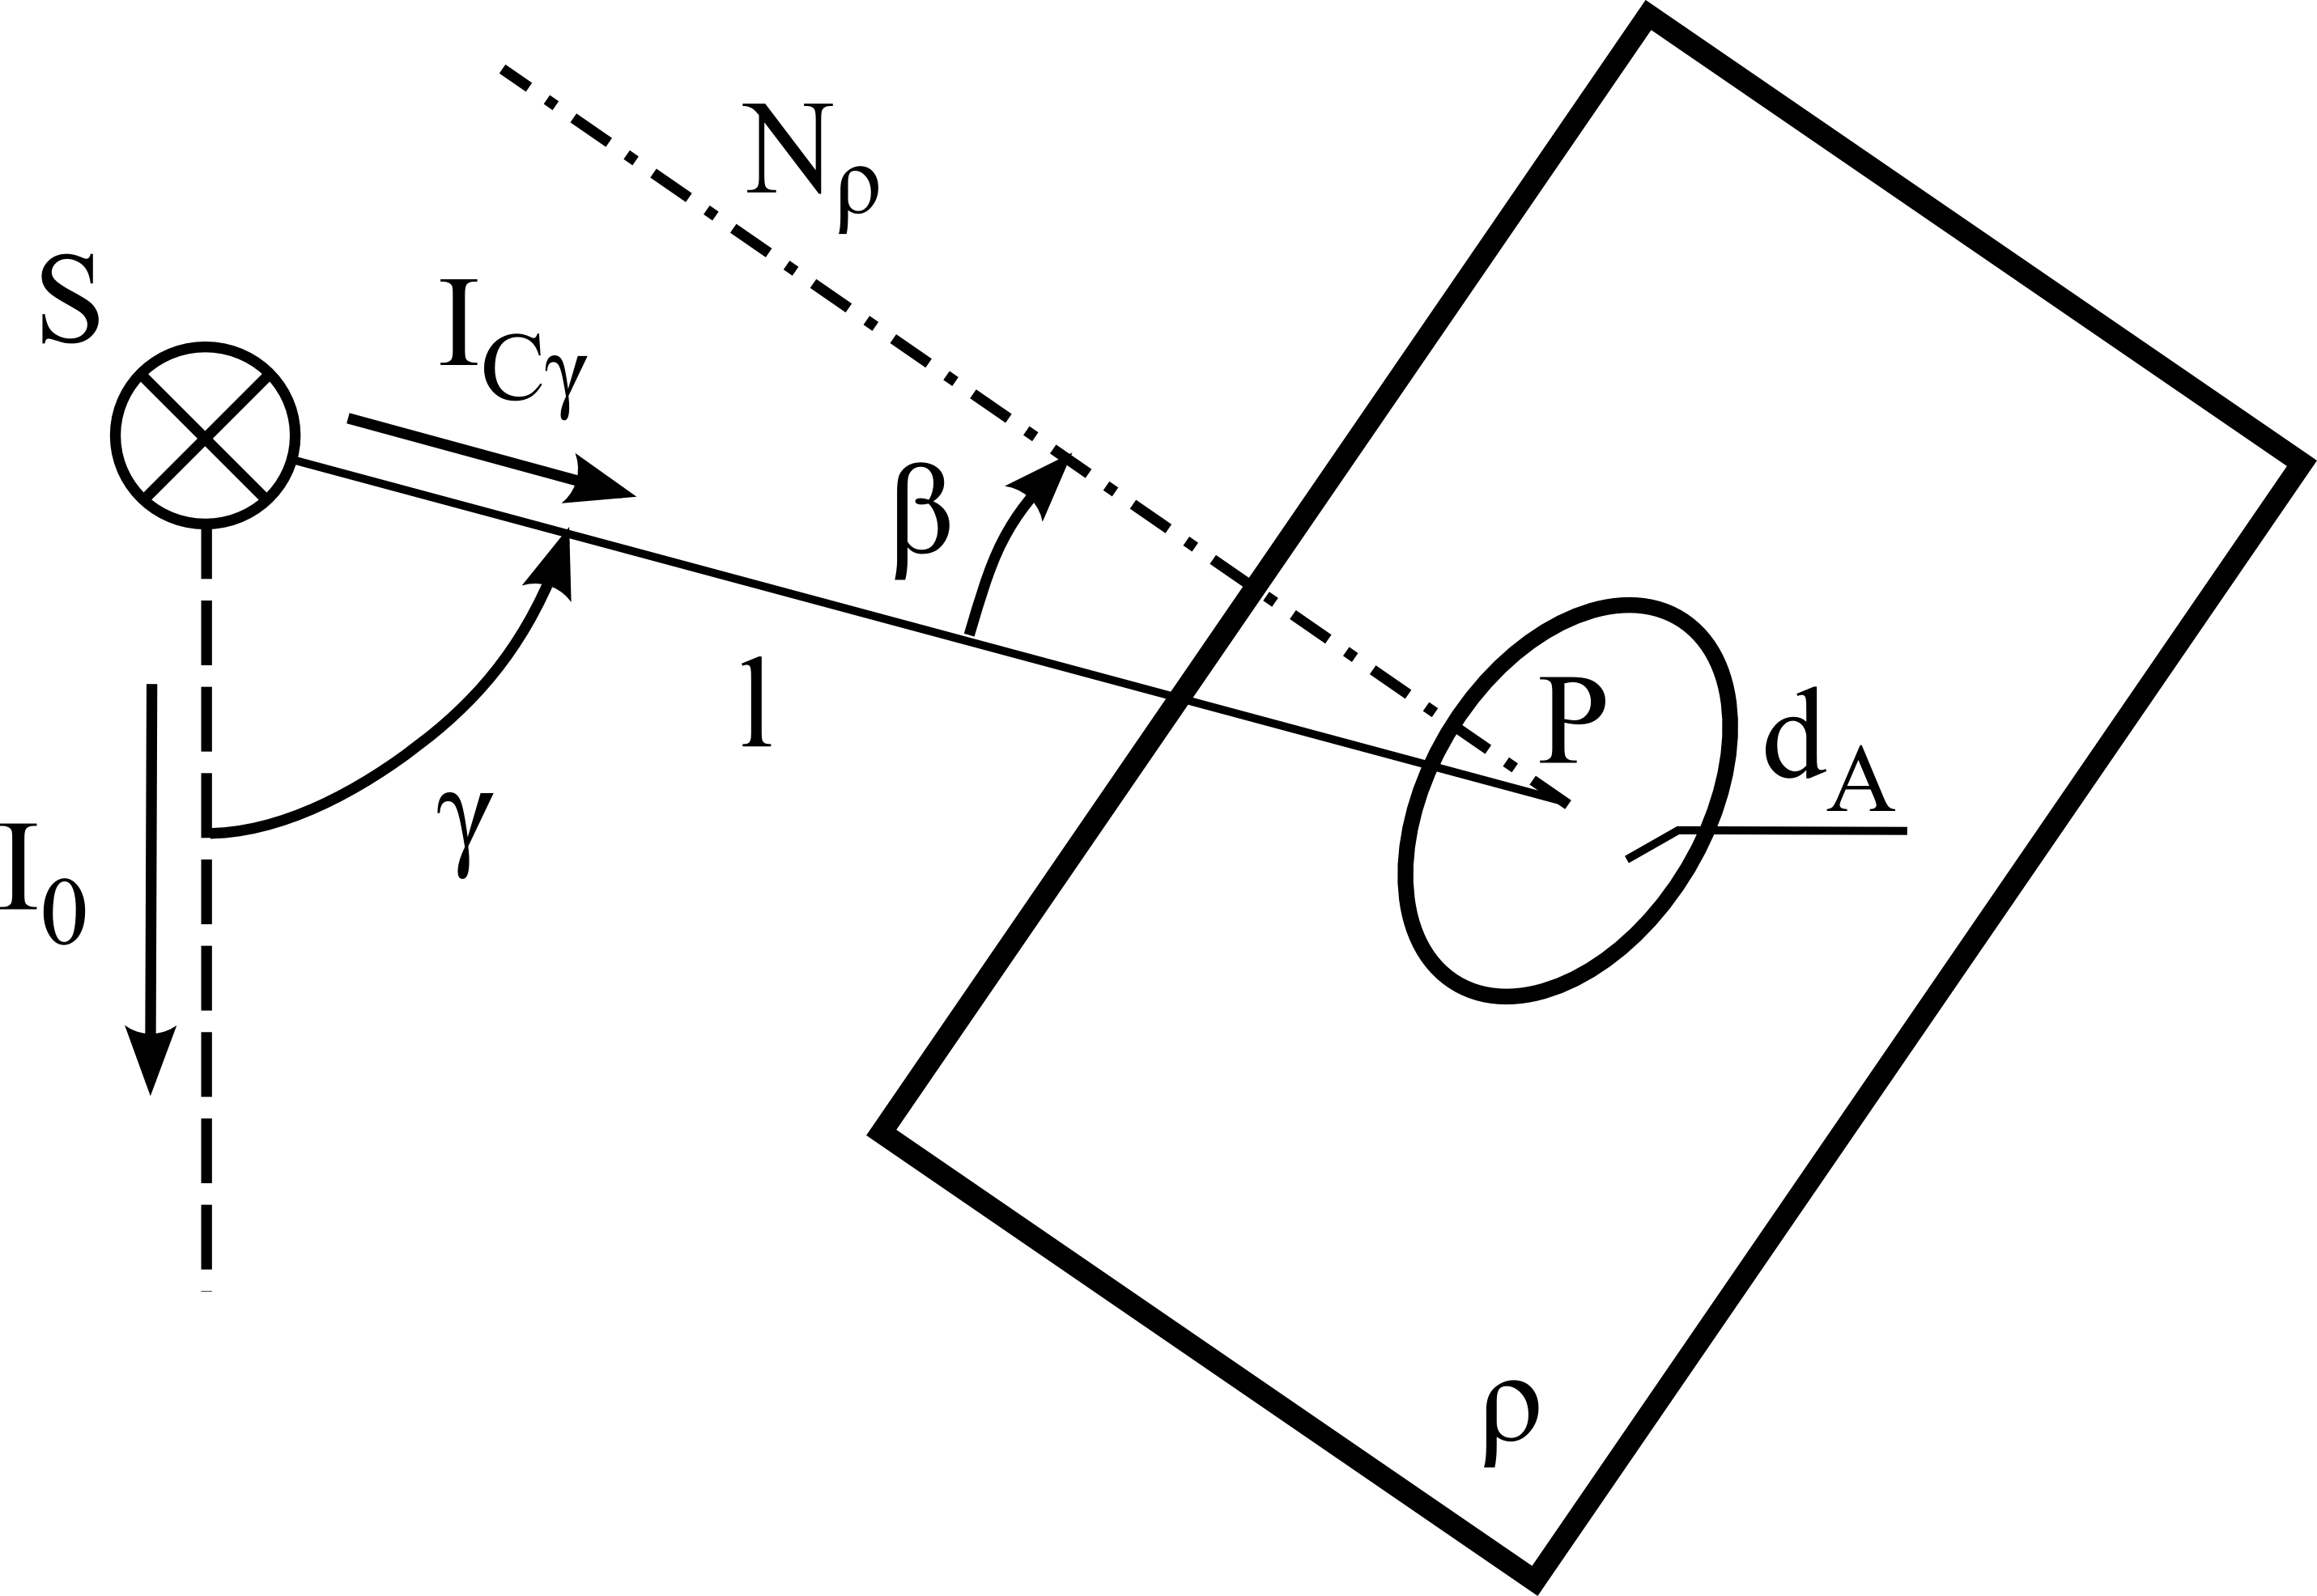
\includegraphics[width=160pt]{315_osvetlenost_bodovym_zdrojem_2}
  \caption{Light source $S$ illuminates point $P$ of plane $\rho$.}
  \label{fig:osv}
\end{figure}

Luminous intensity curves can be found in Eulumdat files of luminaires to enable light scene calculations. Most Eulumdat files of indoor luminaires use the $C-\gamma$ angular coordinate system (Figure~\ref{fig:cgamma}).

\begin{figure}[htb]
  \centering
  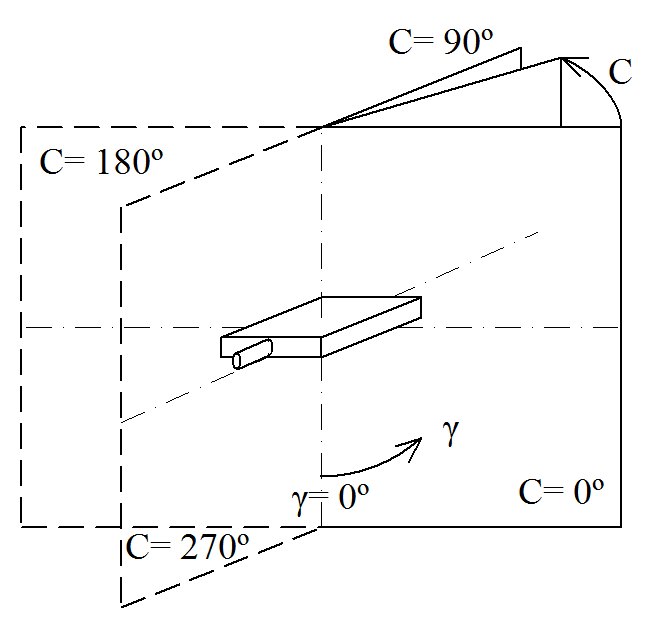
\includegraphics[width=150pt]{Cgama}
  \caption{$C-\gamma$ polar coordinate system with luminaire in center}
  \label{fig:cgamma}
\end{figure}

To bring simulation results closer to real conditions, interaction of light and surfaces has to be included into calculations. Due to the model room's geometric configuration, light reflection affects the light scene the most in this project. Walls, ceiling and floor are becoming secondary light sources after light impact. Using the finite element method, surfaces of the model room are divided into smaller facets each becoming a point light source illuminating other facets leading to multiple reflections (Figure~\ref{fig:difRefl}). During each light reflection a portion of incident luminous flux is absorbed by the surface defined by reflectance value $\rho$. After several reflections the reflected luminous flux becomes negligible.

\begin{figure}[htb]
  \centering
  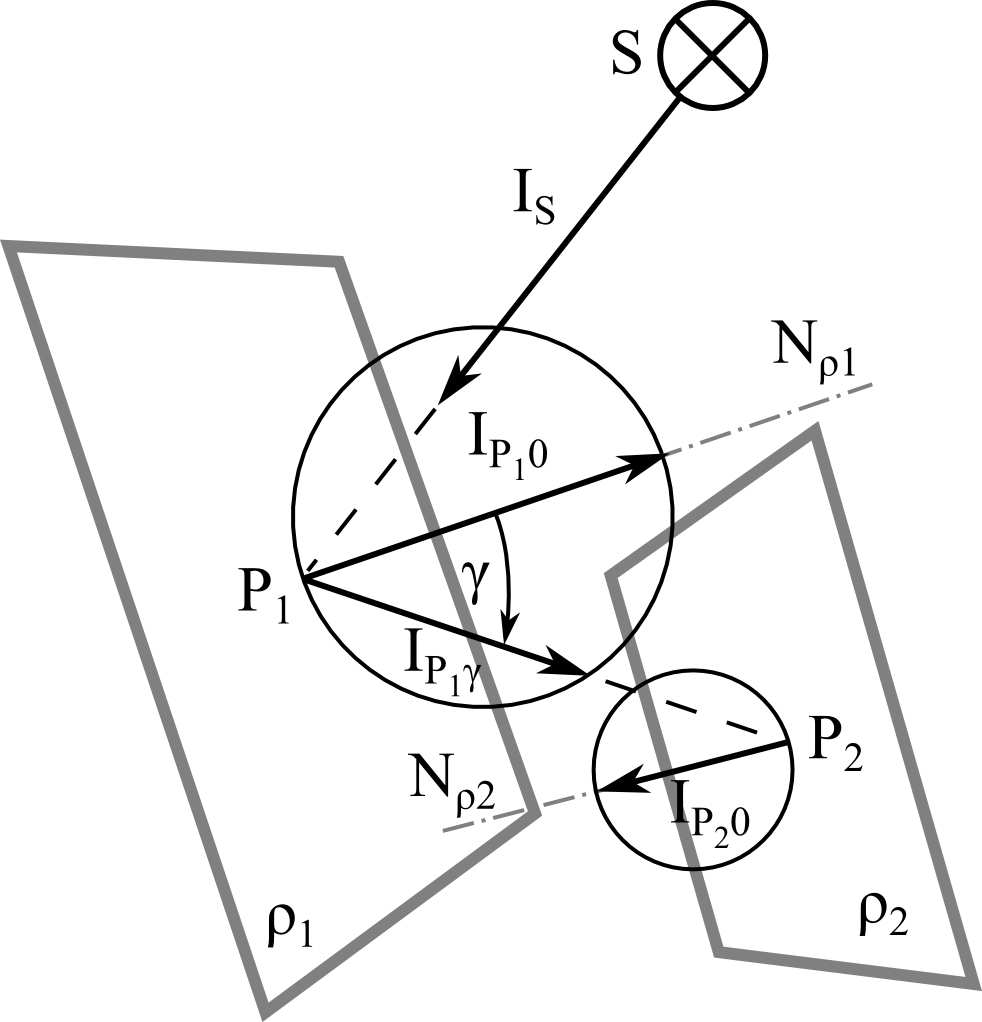
\includegraphics[width=136pt]{diffuseReflection}
  \caption{Multiple reflections between planes $\rho1$ and $\rho2$ with Lambertian reflectance}
  \label{fig:difRefl}
\end{figure}

Most common indoor wall and ceiling surfaces exhibit near Lambertian (diffuse) reflectance. The spatial luminous intensity distribution of purely Lambertian surfaces is dependent only on the referential luminous intensity $I_{0}$ and on angle~$\gamma$ between the surface's normal and the observed direction of the outgoing light ray (Equation~\ref{eq:Igamma}). $I_{0}$ is the luminous intensity of a surface into direction $\gamma=0^{\circ}$, i.e. the surface's normal ($I_{P_{1}0}$ for surface $\rho_1$ and $I_{P_{2}0}$ for surface $\rho_2$ in Figure~\ref{fig:difRefl}). For simplification reasons all surfaces have been chosen to exhibit purely diffuse reflection, including the floor of the model room. Such surfaces become secondary light sources of luminous intensity in direction $\gamma=0^{\circ}$ according to \cite{Habel}:

\begin{equation}
I_{0}=\frac{\rho \cdot E \cdot dA}{\pi} \quad \mathrm{(cd;-,lx,m^{2})}
\label{eq:lumInt}
\end{equation}

where:
\begin{description}
	\item[$I_{0}$] is the referential luminous intensity of the facet in direction of the facet's normal,
	\item[$\rho$] is the facet's integral reflectance,
	\item[$E$] is the facet's illuminance,
	\item[$dA$] is the facet's area.
\end{description}

It must be noted, that luminous intensity is defined only for point light sources. The larger the facet's area $dA$, the lower the calculation accuracy~\cite{handbook}.

After obtaining $I_{0}$, the luminous intensity curve of a facet of Lambertian reflectance will be:

\begin{equation}
I_{\gamma}=I_{0} \cdot \cos(\gamma) \quad \mathrm{(cd;cd,-)}
\label{eq:Igamma}
\end{equation}

where:
\begin{description}
	\item[$I_{\gamma}$] is the luminous intensity in direction $\gamma$.
%	\item[$I_{0}$] is the luminous intensity in direction of facet's normal,
%	\item[$\gamma$] is the angle between the facet's normal and the required direction.
\end{description}

Calculating resulting luminous intensities $I_{0}$ of all available facets of the model room becoming secondary light sources after light impact is achieved in several passes depending on the required amount of reflections. For each facet of the model room light flux cast by primary light sources and the remaining facets is calculated during a single pass. The newly obtained values can then be used later for another pass or for the final reference plane illuminance calculations.

%\begin{itemize}
%	\item Primary light sources emit light incident on visible facets (direct illumination). Initial illuminance $E_{0\rho}$ of facet $\rho$ is obtained by summing up all partial illuminances from all primary light sources (Equation~\ref{eq:illSum}).
%	\item Facets become secondary light sources. Their spacial luminous intensity distributions can be obtained from Equation~\ref{eq:lumInt} and \ref{eq:Igamma} using initial illuminance $E_{0}$. Facet's~$\rho$ illuminance~$E_{1\rho}$ is obtained using Equation~\ref{eq:illSum} and all visible facets as light sources.
%	\item 
%\end{itemize}
%
%First of all primary light sources emit light incident on those facets. Using Equation~\ref{eq:illSum} facets' illuminances can be calculated. 